\textbf{2. Perturbation}.  The energy absorption rate $\propto \chi_0 (q, \omega)$ from the perturbation $(q, \omega)$. At zero temperature $\chi_0(T=0)''$ could be rewritten as
\begin{equation*}
	\chi_0''(q,\omega) = \frac{m}{2|q|} \left(
		\theta(- \xi_{k_-}) - \theta(-\xi_{k_+})
	\right),
	\hspace{10 mm} 
	\xi_k = \frac{\hbar^2 k^2}{2m}  - \frac{\hbar^2 \kF^2}{2m},
	\hspace{5 mm} 
	k_{\pm} = \frac{2 m \omega + q^2}{2q},
\end{equation*}
which completely defines regions with non-zero absorption. Let's find conditions for the boundaries (in units of $\kF$ and $\varepsilon_\text{F}$)
\begin{equation*}
	\left\{\begin{aligned}
	    \kF^2 - k_-^2 &> 0 \\
	    \kF^2 - k_+^2 &< 0 \\
	\end{aligned}\right.
	\hspace{0.5cm} \Rightarrow \hspace{0.5cm}
	\left\{\begin{aligned}
	    &q - \frac{1}{2}q^2  < \omega < q + \frac{1}{2} q^2, &0 < q< 2 \\
	    &-q + \frac{1}{2} q^2   < \omega < q + \frac{1}{2} q^2,  &q > 2
	\end{aligned}\right.
\end{equation*}
, which, taking into account symmetry $\chi_0''(q) = \chi_0''(-q)$, leads to (fig. \ref{fig:12_1}). 
Here we see well defined sharp $\omega(q)$ at $q \ll \kF$ (in contrast to 2D/3D case with macroscopic Fermi surface).


\begin{figure}[h]
    \centering
    \addletter{80}{a}
    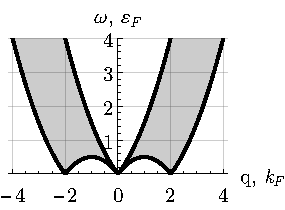
\includegraphics{imgs/mb12_1.pdf}
    \hspace{10 mm} 
    \addletter{80}{b}
	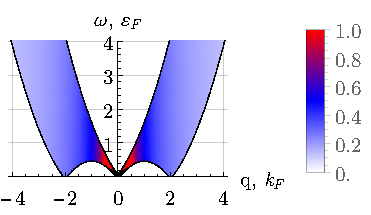
\includegraphics{imgs/mb12_2.pdf}
    \caption{a) Nonzero energy absorption rate regions.  b) The density response function $\chi$ of the weak interacting system. }
    \label{fig:12_1}
\end{figure}
